% Template for the submission to:
%   The Annals of Applied Statistics    [AOAS]
%
%%%%%%%%%%%%%%%%%%%%%%%%%%%%%%%%%%%%%%%%%%%%%%
%% In this template, the places where you   %%
%% need to fill in your information are     %%
%% indicated by '???'.                      %%
%%                                          %%
%% Please do not use \input{...} to include %%
%% other tex files. Submit your LaTeX       %%
%% manuscript as one .tex document.         %%
%%%%%%%%%%%%%%%%%%%%%%%%%%%%%%%%%%%%%%%%%%%%%%

\documentclass[aoas,preprint]{imsart}

%% Packages
\RequirePackage{amsthm,amsmath,amsfonts,amssymb}
\RequirePackage[authoryear]{natbib}
\usepackage{graphicx}
\usepackage{bm}
\usepackage{siunitx}
\usepackage{booktabs}
\usepackage{xcolor}
\usepackage{float}
\usepackage{commath}
\usepackage{fancybox}
\usepackage{tikz}
\usepackage{hyperref}
\usepackage{url}
%\RequirePackage[colorlinks,citecolor=blue,urlcolor=blue]{hyperref}
%\RequirePackage{graphicx}% uncomment this for including figures

\startlocaldefs
%%%%%%%%%%%%%%%%%%%%%%%%%%%%%%%%%%%%%%%%%%%%%%
%%                                          %%
%% Uncomment next line to change            %%
%% the type of equation numbering           %%
%%                                          %%
%%%%%%%%%%%%%%%%%%%%%%%%%%%%%%%%%%%%%%%%%%%%%%
%\numberwithin{equation}{section}
%%%%%%%%%%%%%%%%%%%%%%%%%%%%%%%%%%%%%%%%%%%%%%
%%                                          %%
%% For Axiom, Claim, Corollary, Hypothezis, %%
%% Lemma, Theorem, Proposition              %%
%% use \theoremstyle{plain}                 %%
%%                                          %%
%%%%%%%%%%%%%%%%%%%%%%%%%%%%%%%%%%%%%%%%%%%%%%
%\theoremstyle{plain}
%\newtheorem{???}{???}
%\newtheorem*{???}{???}
%\newtheorem{???}{???}[???]
%\newtheorem{???}[???]{???}
%%%%%%%%%%%%%%%%%%%%%%%%%%%%%%%%%%%%%%%%%%%%%%
%%                                          %%
%% For Assumption, Definition, Example,     %%
%% Notation, Property, Remark, Fact         %%
%% use \theoremstyle{remark}                %%
%%                                          %%
%%%%%%%%%%%%%%%%%%%%%%%%%%%%%%%%%%%%%%%%%%%%%%
%\theoremstyle{remark}
%\newtheorem{???}{???}
%\newtheorem*{???}{???}
%\newtheorem{???}{???}[???]
%\newtheorem{???}[???]{???}
%%%%%%%%%%%%%%%%%%%%%%%%%%%%%%%%%%%%%%%%%%%%%%
%% Please put your definitions here:        %%
%%%%%%%%%%%%%%%%%%%%%%%%%%%%%%%%%%%%%%%%%%%%%%

\endlocaldefs

\begin{document}

\begin{frontmatter}
%%%%%%%%%%%%%%%%%%%%%%%%%%%%%%%%%%%%%%%%%%%%%%
%%                                          %%
%% Enter the title of your article here     %%
%%                                          %%
%%%%%%%%%%%%%%%%%%%%%%%%%%%%%%%%%%%%%%%%%%%%%%
\title{Supplementary Material (1/3): Data Statistics}
%\title{A sample article title with some additional note\thanksref{T1}}
\runtitle{Supplementary Material}
%\thankstext{T1}{A sample of additional note to the title.}

\begin{aug}
%%%%%%%%%%%%%%%%%%%%%%%%%%%%%%%%%%%%%%%%%%%%%%
%%Only one address is permitted per author. %%
%%Only division, organization and e-mail is %%
%%included in the address.                  %%
%%Additional information can be included in %%
%%the Acknowledgments section if necessary. %%
%%%%%%%%%%%%%%%%%%%%%%%%%%%%%%%%%%%%%%%%%%%%%%
\author[A]{\fnms{Renzo} \snm{Caballero}\ead[label=e1]{Renzo.CaballeroRosas@kaust.edu.sa}},
\author[B]{\fnms{Ahmed} \snm{Kebaier}\ead[label=e2,mark]{kebaier@math.univ-paris13.fr}},
\author[C]{\fnms{Marco} \snm{Scavino}\ead[label=e3,mark]{mscavino@iesta.edu.uy}}
\and
\author[D]{\fnms{Ra\'ul} \snm{Tempone}\ead[label=e4,mark]{tempone@uq.rwth-aachen.de}}
%%%%%%%%%%%%%%%%%%%%%%%%%%%%%%%%%%%%%%%%%%%%%%
%% Addresses                                %%
%%%%%%%%%%%%%%%%%%%%%%%%%%%%%%%%%%%%%%%%%%%%%%
\address[A]{CEMSE Division, King Abdullah University of Science and Technology, Saudi Arabia, \printead{e1}}
\address[B]{Universit\'e Sorbonne Paris Nord, LAGA, CNRS, UMR 7539, F-93430, Villetaneuse, France, \printead{e2}}
\address[C]{Instituto de Estad\'{\i}stica (IESTA), Universidad de la Rep\'ublica, Montevideo, Uruguay, \printead{e3}}
\address[D]{Chair of Mathematics for Uncertainty Quantification, RWTH Aachen University, Germany, \printead{e4}}
\end{aug}

\begin{abstract}
In this material, we provide statistical analysis from the data. This analysis was used to construct appropriate SDE models.
\end{abstract}

\begin{keyword}
\kwd{Wind Power}
\kwd{Probabilistic Forecasting}
\kwd{Stochastic Differential Equations}
\kwd{Lamperti Transform}
\kwd{Numerical Optimization}
\kwd{Model Selection}
\kwd{Time-Inhomogeneous Jacobi Diffusion}
\end{keyword}

\end{frontmatter}
%%%%%%%%%%%%%%%%%%%%%%%%%%%%%%%%%%%%%%%%%%%%%%
%% Please use \tableofcontents for articles %%
%% with 50 pages and more                   %%
%%%%%%%%%%%%%%%%%%%%%%%%%%%%%%%%%%%%%%%%%%%%%%
%\tableofcontents

%%%%%%%%%%%%%%%%%%%%%%%%%%%%%%%%%%%%%%%%%%%%%%
%%%% Main text entry area:

\tableofcontents

\section{Seasonality effect}

To guaranty an homogeneous year, we study the Mean Absolute Error (MAE) for each provider and for each day. In Figures (\ref{MAE_pA}), (\ref{MAE_pB}), and (\ref{MAE_pC}), we can see the daily and weekly MAE for the providers A, B, and C, respectively.\\
To compute the vector that we are piloting, we realize the operation
\begin{equation*}
\hat{V}(j) =\frac{1}{145} \sum_{i=1}^{145}|V(i,j)|\quad\text{where}\quad j\in\{1,\dots,147\}.
\end{equation*}
Recall that $V(i,j)$ is the normalized error between the ADME real production and the UTE forecast at time $i$ and for the day $j$.

\begin{figure}[H]
\centering
\includegraphics[width=0.485\textwidth]{plots/mean_errors/prov_A/MAE.eps}
\caption{Daily and weekly for the provider A.}
\label{MAE_pA}
\end{figure}

\begin{figure}[H]
\centering
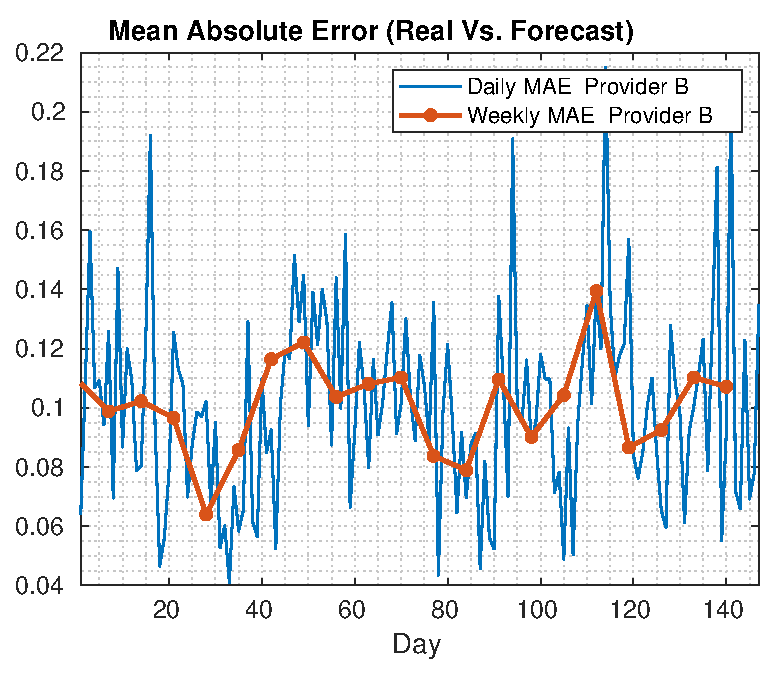
\includegraphics[width=0.485\textwidth]{plots/mean_errors/prov_B/MAE.eps}
\caption{Daily and weekly for the provider B.}
\label{MAE_pB}
\end{figure}

\begin{figure}[H]
\centering
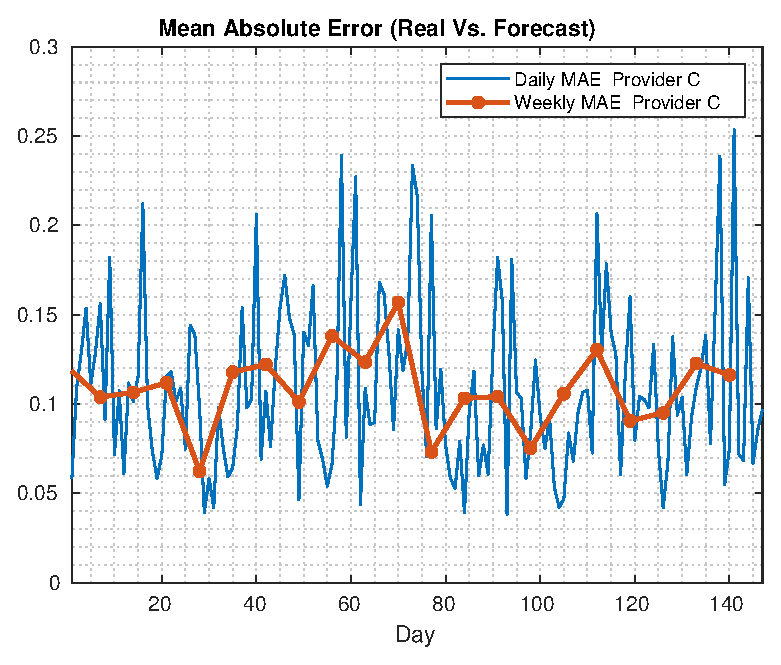
\includegraphics[width=0.485\textwidth]{plots/mean_errors/prov_C/MAE.eps}
\caption{Daily and weekly for the provider C.}
\label{MAE_pC}
\end{figure}

\section{Hourly effect}

We want to see the error throughout the day. We compute the MAE for each provider for each measurement during the day. In Figures (\ref{HMAE_pA}), (\ref{HMAE_pB}), and (\ref{HMAE_pC}), we can see the hourly MAE for the providers A, B, and C, respectively.\\

To compute the vector that we are piloting, we realize the operation
\begin{equation*}
\hat{V}(i) =\frac{1}{147} \sum_{j=1}^{147}|V(i,j)|\quad\text{where}\quad i\in\{1,\dots,145\}.
\end{equation*}
Recall that $V(i,j)$ is the normalized error between the ADME real production and the UTE forecast at time $i$ and for the day $j$.\\

\begin{figure}[H]
\centering
\includegraphics[width=0.485\textwidth]{plots/mean_errors/prov_A/H_MAE.eps}
\caption{MAE along the day for the provider A.}
\label{HMAE_pA}
\end{figure}

\begin{figure}[H]
\centering
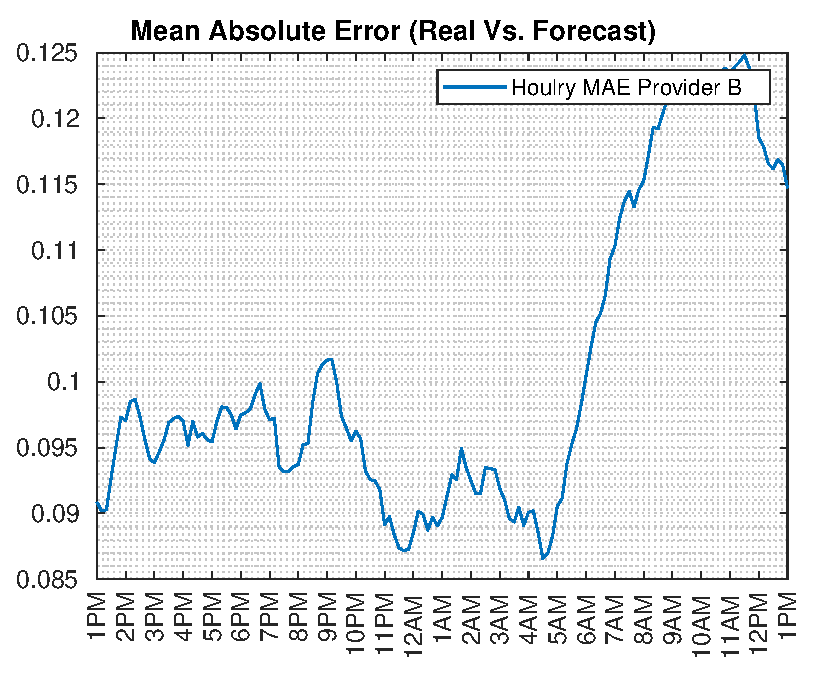
\includegraphics[width=0.485\textwidth]{plots/mean_errors/prov_B/H_MAE.eps}
\caption{MAE along the day for the provider B.}
\label{HMAE_pB}
\end{figure}

\begin{figure}[H]
\centering
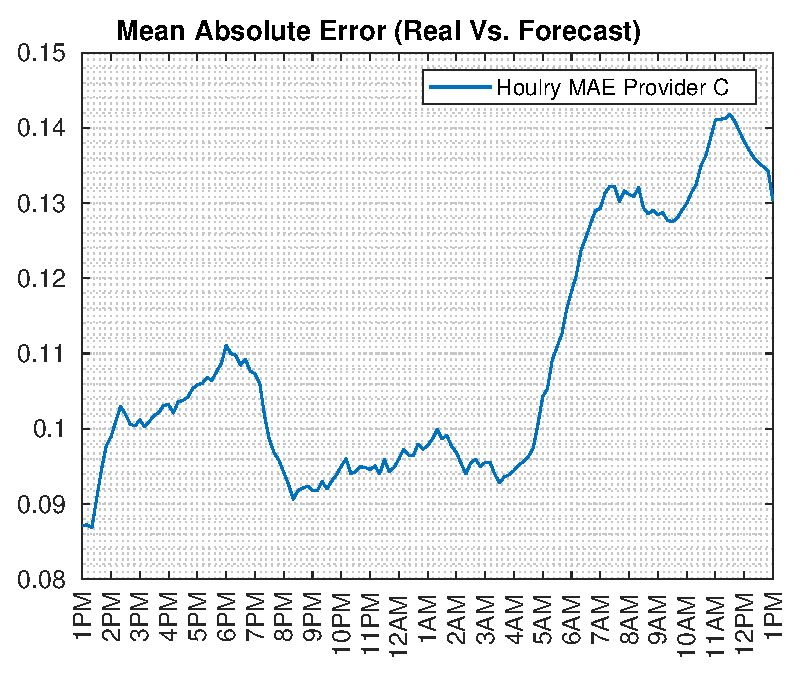
\includegraphics[width=0.485\textwidth]{plots/mean_errors/prov_C/H_MAE.eps}
\caption{MAE along the day for the provider C.}
\label{HMAE_pC}
\end{figure}

\section{Forecast Error Vs Forecast:}

We plot the forecast error as a function of the forecast value for each provider. In Figures (\ref{sA}), (\ref{sB}), and (\ref{sC}), we can see this plots for the providers A, B, and C, respectively.

\begin{figure}[H]
\centering
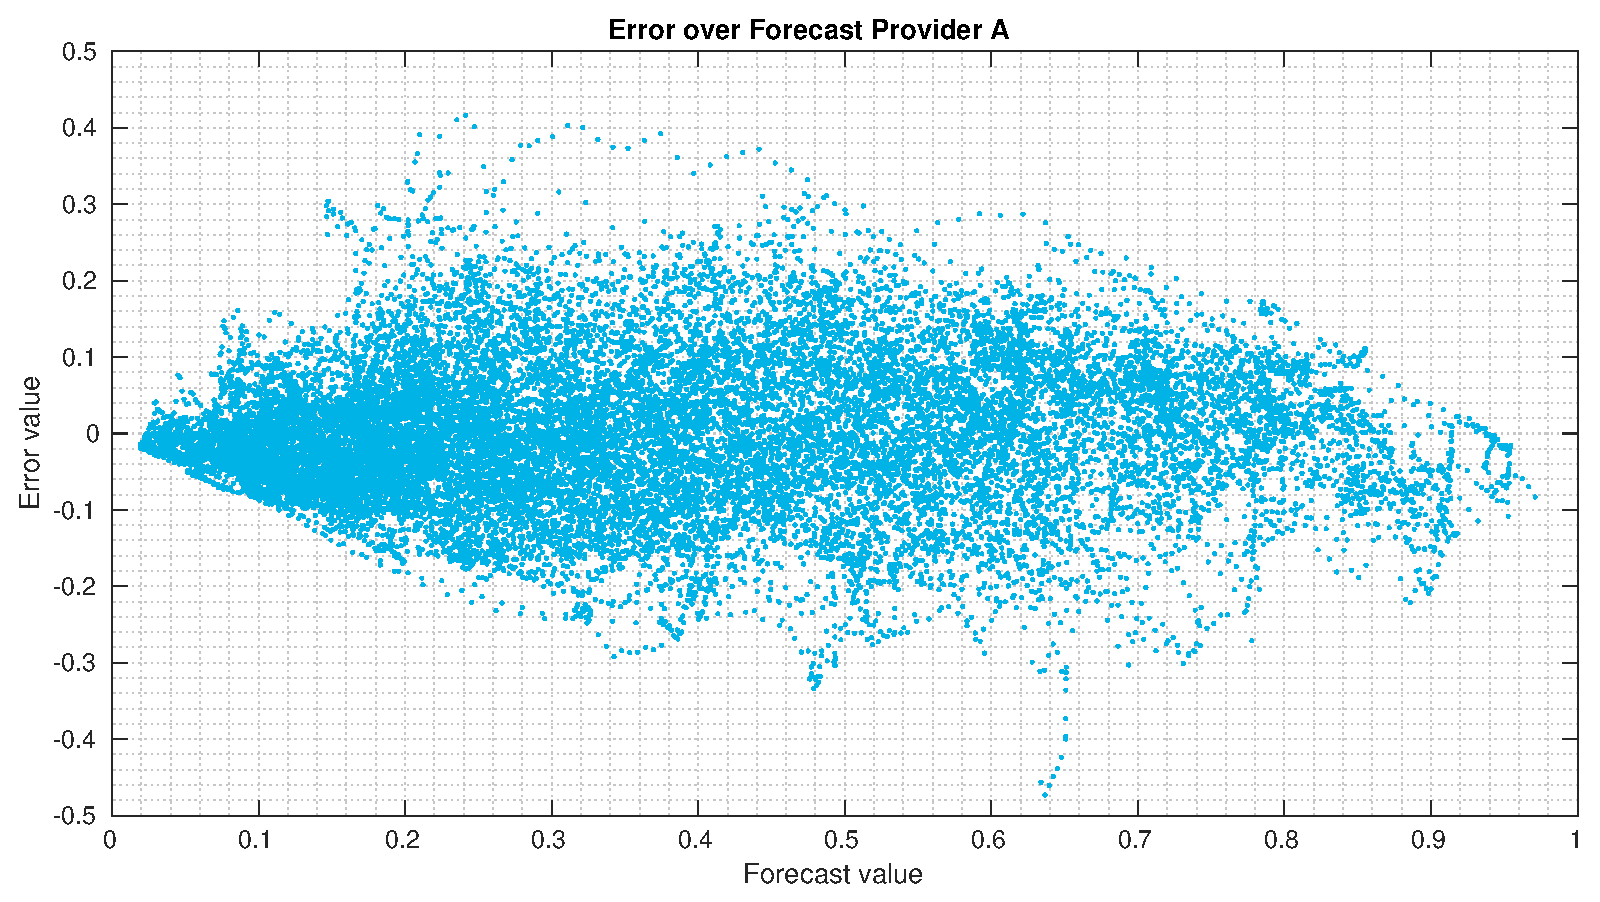
\includegraphics[width=0.8\textwidth]{plots/scatter/prov_A/scatter.eps}
\caption{MAE along the day for the provider A.}
\label{sA}
\end{figure}

\begin{figure}[H]
\centering
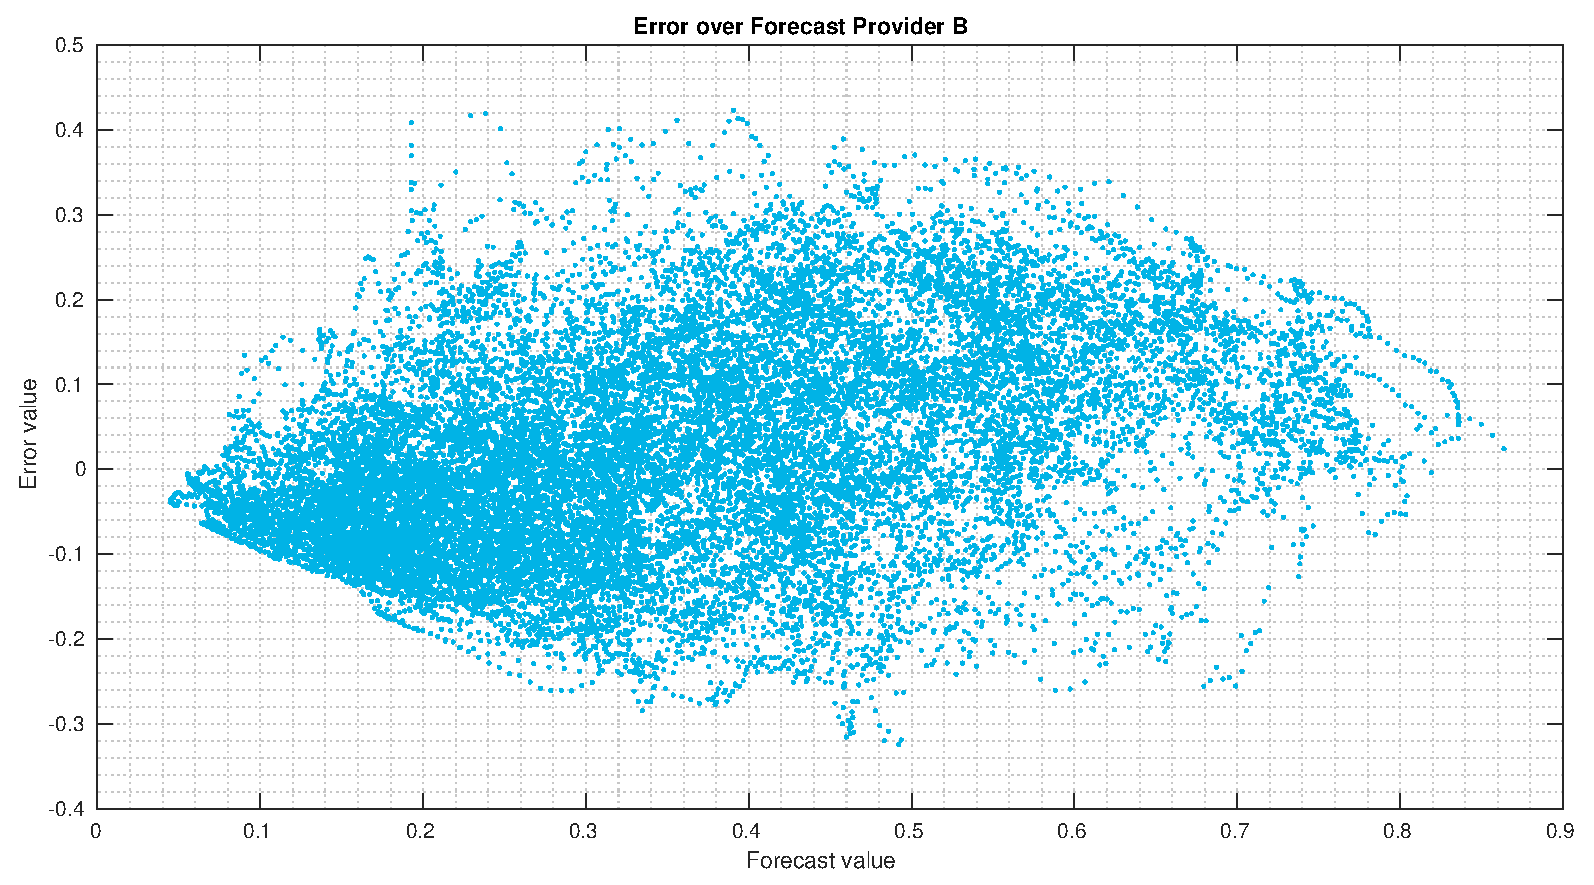
\includegraphics[width=0.8\textwidth]{plots/scatter/prov_B/scatter.eps}
\caption{MAE along the day for the provider B.}
\label{sB}
\end{figure}

\begin{figure}[H]
\centering
\includegraphics[width=0.8\textwidth]{plots/scatter/prov_C/scatter.eps}
\caption{MAE along the day for the provider C.}
\label{sC}
\end{figure}

%%%%%%%%%%%%%%%%%%%%%%%%%%%%%%%%%%%%%%%%%%%%%%
%% Single Appendix:                         %%
%%%%%%%%%%%%%%%%%%%%%%%%%%%%%%%%%%%%%%%%%%%%%%
%\begin{appendix}
%\section*{???}%% if no title is needed, leave empty \section*{}.
%\end{appendix}
%%%%%%%%%%%%%%%%%%%%%%%%%%%%%%%%%%%%%%%%%%%%%%
%% Multiple Appendixes:                     %%
%%%%%%%%%%%%%%%%%%%%%%%%%%%%%%%%%%%%%%%%%%%%%%
%\begin{appendix}
%\section{???}
%
%\section{???}
%
%\end{appendix}

%%%%%%%%%%%%%%%%%%%%%%%%%%%%%%%%%%%%%%%%%%%%%%
%% Support information (funding), if any,   %%
%% should be provided in the                %%
%% Acknowledgements section.                %%
%%%%%%%%%%%%%%%%%%%%%%%%%%%%%%%%%%%%%%%%%%%%%%
% \section*{Acknowledgements}
% The authors would like to thank ...
% 
% The first author was supported by ...
% 
% The second author was supported in part by ...
 
%%%%%%%%%%%%%%%%%%%%%%%%%%%%%%%%%%%%%%%%%%%%%%
%% Supplementary Material, if any, should   %%
%% be provided in {supplement} environment  %%
%% with title inside \textbf{} and short    %%
%% description below.                       %%
%%%%%%%%%%%%%%%%%%%%%%%%%%%%%%%%%%%%%%%%%%%%%%
%\begin{supplement}
%\textbf{???}.
%???.
%\end{supplement}

%%%%%%%%%%%%%%%%%%%%%%%%%%%%%%%%%%%%%%%%%%%%%%%%%%%%%%%%%%%%%
%%                  The Bibliography                       %%
%%                                                         %%
%%  imsart-nameyear.bst  will be used to                   %%
%%  create a .BBL file for submission.                     %%
%%                                                         %%
%%  Note that the displayed Bibliography will not          %%
%%  necessarily be rendered by Latex exactly as specified  %%
%%  in the online Instructions for Authors.                %%
%%                                                         %%
%%  MR numbers will be added by VTeX.                      %%
%%                                                         %%
%%  Use \cite{...} to cite references in text.             %%
%%                                                         %%
%%%%%%%%%%%%%%%%%%%%%%%%%%%%%%%%%%%%%%%%%%%%%%%%%%%%%%%%%%%%%

%% if your bibliography is in bibtex format, uncomment commands:
%\bibliographystyle{imsart-nameyear} % Style BST file
%\bibliography{bibliography}       % Bibliography file (usually '*.bib')

%% or include bibliography directly:
% \begin{thebibliography}{}
% \bibitem[\protect\citeauthoryear{???}{???}]{b1}
% \end{thebibliography}

\end{document}
